\textbf{Beispiel 2}\\ \\
a)\\ \\
Freigeschnittene Teilkörper:
\begin{figure}[h]
	\centering
	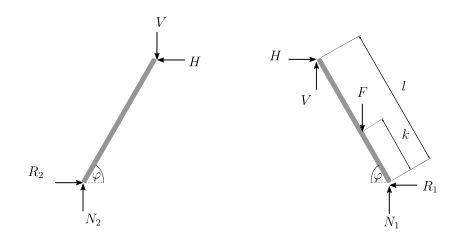
\includegraphics[width= 8cm]{tikz/18_05_2018_2a}
\end{figure}
\newpage
\noindent
b)\\ \\
Die notwendigen Gleichgewichtsgleichungen lautet für den rechten Teil 
\begin{align}
	\textbf{e}_x &: R_1 = H\\
	\textbf{e}_y &: F = V + N_1\\
	\textbf{e}_z &: k\cos(\varphi)F = Vl\cos(\varphi) + Hl\sin(\varphi)
\end{align}
und den linken Teil
\begin{align*}
	\textbf{e}_x &: R_2 = H\\
	\textbf{e}_y &: N_2 = V\\
	\textbf{e}_z &: Hl\sin(\varphi) = Vl\cos(\varphi)
\end{align*}
Durch gezieltes Umformen dieser Gleichung erhält man für die Bodenkontaktkräfte
\begin{align*}
	R &= F\frac{k}{2l\tan(\varphi)} \\
	N_1 &= F\frac{2l - k}{2l} \\
	N_2 &= F\frac{k}{2l}
\end{align*}
c)\\ \\
Da es sich um Haftreibung handelt lautet die Bedingung für den rechten Teil
\begin{align*}
	\mu \geq \frac{R_1}{N_1} &= \frac{F\frac{k}{2l\tan(\varphi)}}{F\frac{2l - k}{2l}} = \frac{k}{(2l - k)\tan(\alpha)}
\end{align*}
und den linken Teil
\[
	\mu \geq \frac{R_2}{N_2} = \frac{F\frac{k}{2l\tan(\varphi)}}{F\frac{k}{2l}} = \frac{1}{\tan(\alpha)}
\]